\documentclass[10pt,a4paper]{article}
\usepackage[margin=20mm]{geometry}
\usepackage[T1]{fontenc}
\usepackage[utf8]{inputenc}
\usepackage{lmodern,microtype,amsmath,amssymb,booktabs,tabularx,graphicx,caption,xcolor,titlesec,fancyhdr,hyperref,xurl}
\setcounter{secnumdepth}{-1}
\definecolor{ink}{HTML}{17252A}\definecolor{teal}{HTML}{176B68}\definecolor{gold}{HTML}{B8892F}
\hypersetup{colorlinks=true,linkcolor=teal,urlcolor=teal,citecolor=teal,pdftitle={Importance Is Not Necessity},pdfauthor={Joseph Maxwell}}
\titleformat{\section}{\Large\bfseries\sffamily\color{ink}}{\thesection}{0.6em}{}
\titleformat{\subsection}{\large\bfseries\sffamily\color{teal}}{\thesubsection}{0.6em}{}
\captionsetup{font=small,labelfont=bf,justification=raggedright,singlelinecheck=false}
\pagestyle{fancy}\fancyhf{}\fancyhead[L]{\small\sffamily MATERIALS ML FAILURE ANALYSIS}\fancyhead[R]{\small\sffamily FINAL QA V4}\fancyfoot[C]{\small\thepage}\setlength{\headheight}{15pt}
\setlength{\parindent}{0pt}\setlength{\parskip}{5pt plus 1pt}\setlength{\emergencystretch}{2em}
\newcommand{\plainbox}[1]{\begin{center}\fcolorbox{teal}{teal!5}{\begin{minipage}{0.92\linewidth}#1\end{minipage}}\end{center}}
\title{Importance Is Not Necessity\\\large Fitted Feature Importance and Retrained Removal Consequence in Materials-Property Models}
\author{Joseph Maxwell\\\small The Systemica Institute, London, United Kingdom\\\small ORCID: \href{https://orcid.org/0009-0002-4070-6035}{0009-0002-4070-6035}\\\small \href{mailto:j.maxwell@systemicainstitute.org}{j.maxwell@systemicainstitute.org}}
\date{Preprint -- August 2026}
\begin{document}\maketitle

\begin{abstract}
Feature importance describes how a fitted predictor uses its inputs. It does not necessarily describe what remains important after the model is retrained without one input. We compared fitted permutation importance with complete retrained-removal consequence on four official Matbench regression tasks. Each task used 142 composition-based Magpie descriptors, five prescribed folds, and the same two-hidden-layer multilayer perceptron. Baseline mean held-out $R^2$ ranged from 0.7504 to 0.9484, so the comparison was made within models showing substantial positive held-out predictive performance. Across all 20 task-fold combinations, the mean Spearman association between permutation importance and removal consequence was 0.0394. Mean top-10 overlap was 0.100. We then repeated the complete 3,440-unit experiment under the same software and hardware environment. All 65,740 compared numeric cells were exactly equal. The disagreement persisted under an exact same-environment execution repeat. This is not external replication. The finding does not show that descriptors are causally irrelevant, physically unnecessary, or universally substitutable. It shows that an importance ranking from a fitted model should not be used as a direct proxy for the consequence of deleting information and allowing the model to adapt.
\end{abstract}

\plainbox{\textbf{This paper in plain language}\par
\textbf{Question:} Does a feature that looks important to a trained model still matter when the model is rebuilt without it?\par
\textbf{Why it matters:} A fitted ranking can be mistaken for a ranking of what the learning problem uniquely requires.\par
\textbf{What we did:} We ranked 142 materials descriptors by fitted permutation importance, then removed descriptors and completely retrained the network.\par
\textbf{What we found:} Across four Matbench tasks, the two rankings had a mean Spearman correlation of only \textbf{0.0394}.\par
\textbf{What it does not mean:} The result does not establish physical causality or prove that any descriptor is universally unnecessary.}

\noindent\textbf{Three ways to read this paper.} \textbf{Just want the answer?} Read the box, Figure~\ref{fig:rank}, and the Conclusion. \textbf{Want the experiment?} Read Materials and Methods plus Results. \textbf{Want to audit it?} Follow the public scientific-method specification, accepted evidence, and reconstruction package.

\section{1. Introduction}
A fitted model can be inspected by disturbing one input while leaving the trained parameters fixed. Permutation importance follows this logic. If shuffling a descriptor worsens held-out prediction, the fitted model relied on that descriptor in its current form.

Retrained removal asks a different question. The descriptor is deleted before fitting, the preprocessing and model are rebuilt, and the reduced model is trained again. The result measures whether the remaining representation can compensate for the missing input.

This distinction matters in materials informatics because composition descriptors are strongly structured and often correlated. Several descriptors may encode related chemical trends. A model can rely on one member of such a set while an independently retrained model shifts its reliance to the others. Conversely, a descriptor with modest fitted importance can become costly to remove if its information is not easily recovered.

``Necessity'' in the title is shorthand for consequence under retraining within the declared representation. The experiment does not test physical necessity in nature.

We therefore asked one narrow question: \emph{does fitted permutation importance agree with complete retrained-removal consequence under one fixed materials-ML protocol?}

This study contributes three measurements. First, it compares fitted permutation importance and complete retrained removal on the same tasks, folds, descriptors, and model family. Second, it resolves the comparison at both individual-descriptor and predeclared descriptor-group levels. Third, it repeats the complete 3,440-unit route in the same environment and compares every claim-relevant numeric output.

We do not propose a new feature-importance estimator. The contribution is the empirical measurement of how strongly fitted permutation importance and complete retrained-removal consequence disagree under a fixed materials-informatics protocol, together with an exact same-environment repeat of that measurement.

\begin{table}[htbp]\centering\small
\caption{Adjacent methods answer related but non-identical questions.}
\begin{tabularx}{\linewidth}{@{}p{0.26\linewidth}X p{0.23\linewidth}@{}}\toprule
Method & Primary question & Role here\\\midrule
Fitted permutation importance & What inputs does this trained predictor use? & First measurement\\
Leave-one-covariate-out or retraining & What changes after an input is removed and the model refitted? & Second measurement\\
Feature selection & Which subset optimises a declared criterion? & Related, not the target question\\
This study & Do the two descriptor accounts agree under one frozen materials protocol? & Paired comparison and repeat\\\bottomrule
\end{tabularx}\end{table}

\section{2. Materials and Methods}
\subsection{2.1 Tasks and representation}
We used four regression tasks from Matbench v0.1: \texttt{matbench\_mp\_e\_form} (132,752 records), \texttt{matbench\_mp\_gap} (106,113), \texttt{matbench\_log\_kvrh} (10,987), and \texttt{matbench\_log\_gvrh} (10,987). These represent formation energy per atom, band gap, log bulk modulus, and log shear modulus. The route consumed the targets supplied by Matbench; it did not apply an additional target transformation.

We used the five official Matbench folds. No rows were filtered or subsampled after task loading. Each composition was featurised with Matminer's Magpie elemental-property statistics, stoichiometric norms, and average valence-orbital fractions. The ordered frozen representation contained 142 numeric descriptors.

\subsection{2.2 Model and training specification}
Every fit used a scikit-learn 1.8.0 pipeline. Median imputation and standardisation were fitted only on the training portion of each official fold. They were refitted for every removal model. Targets were neither scaled nor inverse-transformed.

\begin{table}[htbp]\centering\small
\caption{Frozen multilayer-perceptron specification. ``Default'' means the constructor default under the bound scikit-learn 1.8.0 environment.}
\begin{tabularx}{\linewidth}{@{}p{0.32\linewidth}X@{}}\toprule
Parameter & Value\\\midrule
Estimator & \texttt{MLPRegressor}; input--128--64--1\\
Activation; solver; loss & ReLU; Adam; squared error (defaults)\\
Learning rate & Initial $10^{-3}$; constant schedule (default)\\
Batching & \texttt{auto}, i.e. $\min(200,n_{\mathrm{train}})$ (default)\\
Stopping & 300 maximum iterations; early stopping; 15\% internal validation; patience 20; tolerance $10^{-4}$\\
Regularisation & L2 coefficient $\alpha=10^{-4}$; no dropout layer\\
Randomness & \texttt{random\_state=11}; training shuffle enabled (default)\\
Parallelism & Two process workers; one numerical thread per scientific unit\\
Software & Python 3.14.0; NumPy 2.4.4; SciPy 1.17.1; scikit-learn 1.8.0; Matminer 0.10.1\\\bottomrule
\end{tabularx}\end{table}

The baseline input dimension was 142. Individual-removal models used 141 inputs. Group-removal dimensions depended on the size of the predeclared group. No custom weight initializer was configured; initialization was internal to the bound scikit-learn estimator.

\subsection{2.3 Fitted permutation importance}
For each held-out fold, we independently shuffled one descriptor column and evaluated the unchanged fitted model. Five permutations were generated per descriptor. Each permutation seed was derived from the complete unit identity, feature index, and repetition by SHA-256. We recorded the increase in mean absolute error (MAE) and loss in $R^2$, then averaged over the five permutations. The primary rank comparison used mean MAE increase.

\subsection{2.4 Complete retrained removal}
For each descriptor, we deleted its column from both training and held-out matrices. We then rebuilt the imputation, scaling, and MLP pipeline from the beginning. The same procedure was applied to 29 frozen groups. Those groups combined the six Magpie summary statistics for each elemental property, retained each stoichiometric norm as a separate group, and combined the average valence-orbital features.

Removal consequence was defined as
\[
\Delta \mathrm{MAE}_{\mathrm{remove}}=\mathrm{MAE}_{\mathrm{reduced}}-\mathrm{MAE}_{\mathrm{full}}.
\]
A positive value means deletion worsened held-out MAE. A negative value means the reduced model improved.

\subsection{2.5 Statistical comparison}
Within each task-fold pair, we calculated Spearman's rank correlation between the 142 permutation-MAE increases and the 142 retrained-removal MAE changes using SciPy 1.17.1. Ties received average ranks. We also compared the sets containing the $k$ largest values, for $k=5,10,20$.

For the top-10 reference, two independent random rankings select 10 descriptors from 142. Their overlap follows a hypergeometric distribution with $N=142$, $K=10$, and $n=10$. The expected overlap fraction is $10/142=0.07042$. Under an independent-random-ranking reference model, the probability of total overlap at least this large is 0.0659. Because cross-validation folds are not independent experimental replicates, this value is used only as a descriptive reference rather than an inferential significance test.

MAE and $R^2$ were calculated with scikit-learn 1.8.0. For $R^2$, the reference sum of squares uses the mean of the evaluated held-out targets.

\subsection{2.6 Same-environment repeat}
The fresh execution and repeat had different execution identities but identical protocol, feature registry, ordered plan, code, dependencies, and fold data. Each contained 3,440 independently fitted units. The comparison required exact semantic coverage and compared numeric values with an absolute tolerance of $10^{-10}$. Execution-specific timestamps and wall times were excluded from semantic identity. Because the model seed, software, protocol, and environment were intentionally held fixed, this repeat tests execution reproducibility under the declared environment. It does not establish robustness to alternative random initialisations, implementations, hardware platforms, model families, or external research groups.

\textbf{Scientific unit:} one complete, independently committable part of the declared experiment. It can contain one fit or several fits depending on the route. In this route, each V0.3 unit contained one complete estimator fit; 3,440 units comprised 20 baseline/perturbation fits, 2,840 individual-removal refits, and 580 group-removal refits. Unit counts are accepted scientific boundaries, not a general measure of computational cost. For contrast, the earlier Matbench V0.2 route had \textbf{20 scientific units representing 120 estimator fits}. The cross-programme scale register reports units, fits, and comparison cells separately.

\section{3. Results}
\subsection{3.1 Baseline predictive carrier}
The mean held-out $R^2$ values across the five folds were 0.948426 for formation energy, 0.808299 for band gap, 0.764881 for log bulk modulus, and 0.750357 for log shear modulus (Figure~\ref{fig:baseline}). The disagreement analysis therefore concerns models with substantial predictive signal, not models that had already failed to carry the target.

\begin{figure}[htbp]\centering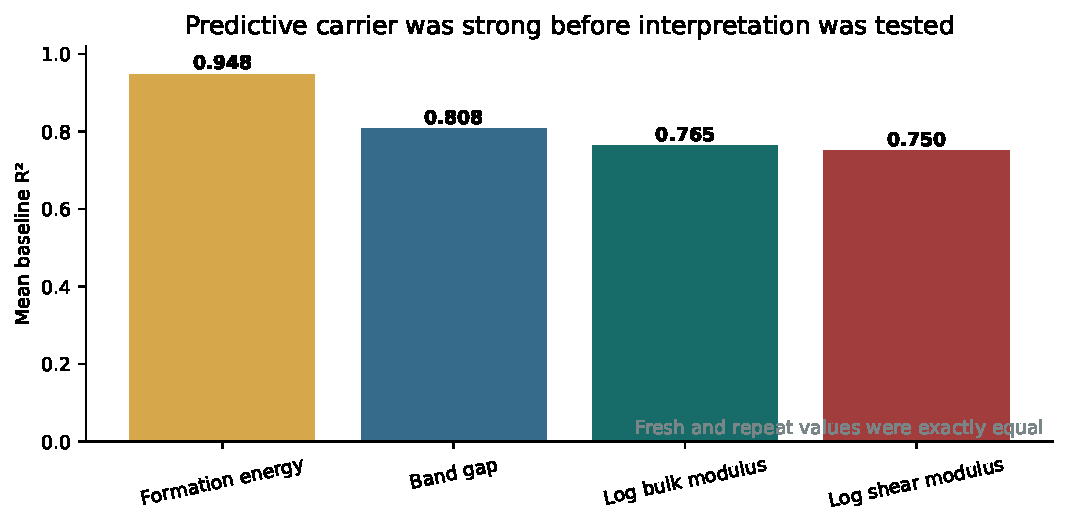
\includegraphics[width=0.82\linewidth]{figures/PAPER_1_BASELINE_REPEATABILITY.pdf}\caption{\textbf{The four benchmark tasks supported substantial positive held-out prediction.} Baseline mean held-out $R^2$ across the five official folds; fresh and repeat values coincide.}\label{fig:baseline}\end{figure}

\subsection{3.2 Rank disagreement}
Across the 20 task-fold comparisons, mean Spearman association was 0.039404. Individual values ranged from $-0.281504$ to $+0.213946$ (Figure~\ref{fig:rank}). The two measurements therefore did not produce a stable common ranking under this protocol.

\begin{figure}[htbp]\centering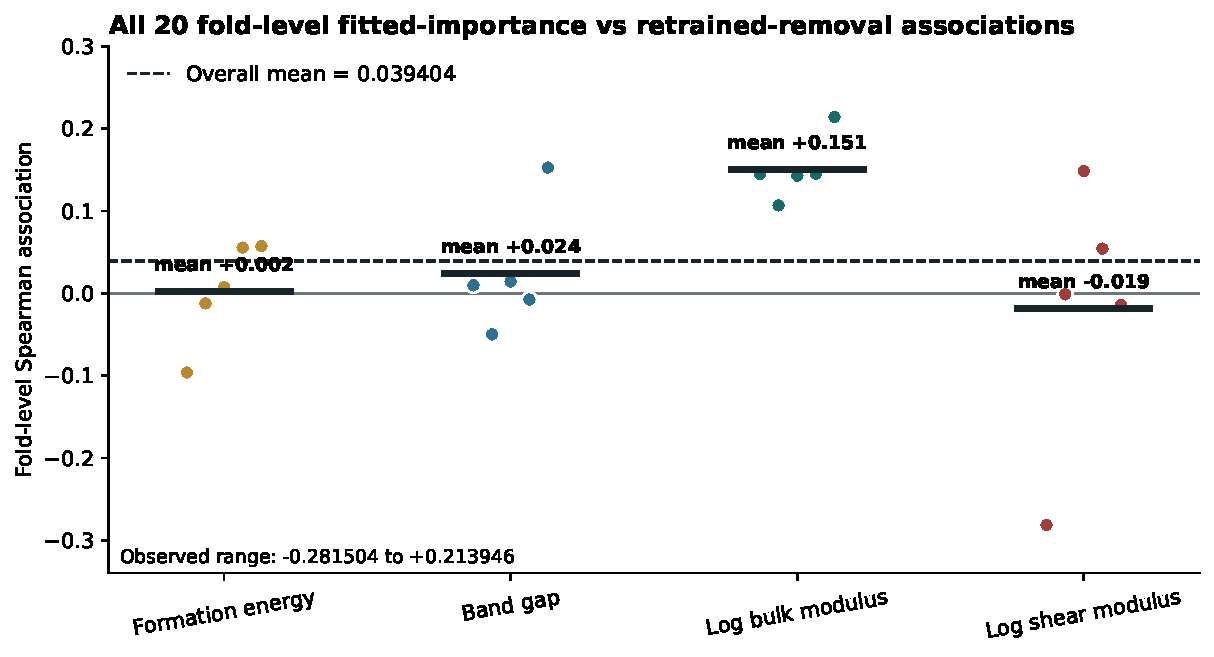
\includegraphics[width=0.92\linewidth]{figures/PAPER_1_FOLD_LEVEL_SPEARMAN_DISTRIBUTION.pdf}\caption{\textbf{The two ways of ranking descriptors mostly disagree.} All 20 fold-level associations between fitted permutation importance and retrained-removal consequence, grouped by task with task means overlaid. The observed range was $-0.281504$ to $+0.213946$ and the overall mean was 0.039404.}\label{fig:rank}\end{figure}

\subsection{3.3 Top-10 reference}
Mean top-10 overlap was 0.100, equivalent to one common descriptor per fold on average. The random-ranking expectation was 0.07042. Under the independent-random-ranking reference, the one-sided probability of a total overlap at least as large as observed was 0.0659 (Figure~\ref{fig:chance}). Cross-validation folds are not independent experimental replicates, so this value is a descriptive reference rather than an inferential significance test.

\begin{figure}[htbp]\centering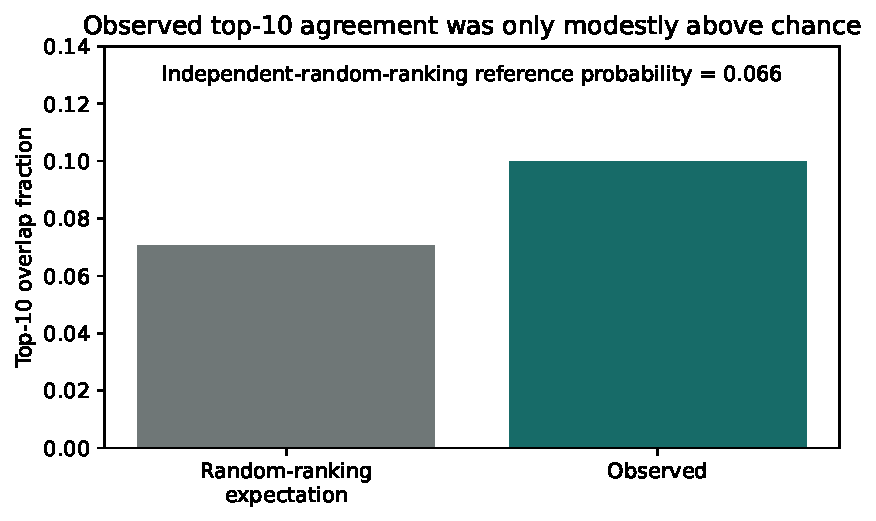
\includegraphics[width=0.50\linewidth]{figures/PAPER_1_TOP10_CHANCE_REFERENCE.pdf}\caption{\textbf{The two methods shared only one top-10 descriptor per fold on average.} Observed top-10 overlap and the independent-random-ranking reference. The displayed value is a descriptive reference probability, not a hypothesis-test $p$-value.}\label{fig:chance}\end{figure}

\subsection{3.4 Individual removals}
The experiment performed 2,840 individual retrained removals: 142 descriptors across four tasks and five folds. Removal improved MAE in 1,781 cases and worsened it in 1,059. Together with the weak rank association, these outcomes show that fitted importance was a poor proxy for retrained-removal consequence under this protocol.

\subsection{3.5 Group-removal materials readout}
The 580 group removals also differed by target (Figure~\ref{fig:groups}). Formation energy and band gap each had positive mean removal consequence for 20 of 29 groups. Shear modulus had six. Bulk modulus had none. For the secondary group-level comparison, individual fitted permutation importances were summed within each frozen descriptor group and ranked against the directly measured group-removal consequence. This was a descriptive grouped comparison rather than direct joint group permutation. The resulting associations were $+0.468$ for formation energy, $+0.369$ for band gap, $-0.262$ for shear, and $-0.189$ for bulk.

These counts do not establish a universal physical hierarchy. They show that retrained dependence was conditional on the property target, representation, and model.

\begin{figure}[htbp]\centering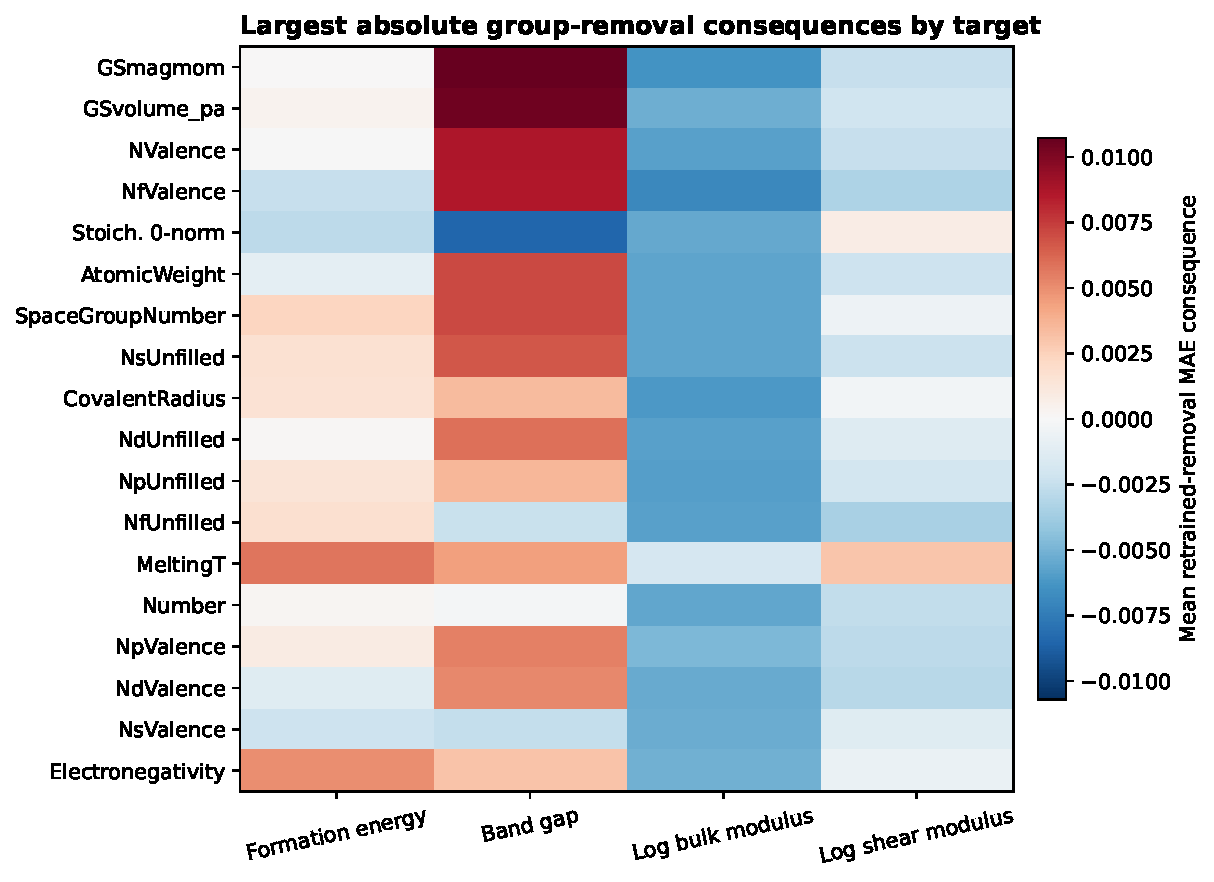
\includegraphics[width=0.96\linewidth]{figures/PAPER_1_GROUP_REMOVAL_TOP18_HEATMAP.pdf}\caption{\textbf{Descriptor-family dependence changed with the material property being predicted.} The display shows the 18 of 29 frozen descriptor groups with the largest absolute mean removal consequence in any target. Positive values indicate worse prediction after removal. All 29 groups were retained in the counts and descriptive rank comparisons.}\label{fig:groups}\end{figure}

\subsection{3.6 Repeat result}
The fresh and repeat executions each sealed 3,440 units. Semantic metadata matched for every unit. Across 65,740 compared numeric cells, the maximum absolute difference was zero. Raw JSON files were not byte-identical because timestamps and measured wall times differed; byte identity was not the scientific equivalence criterion.

\section{4. Discussion}
\subsection{4.1 Two useful measurements, not one failed method}
Permutation importance measures fitted reliance. It is useful when the scientific question concerns the behaviour of a particular trained predictor. Retrained removal measures the consequence of changing the available representation and allowing the model to adapt. It is useful when the question concerns substitutability under a declared training protocol.

The near-zero mean association does not invalidate either method. It shows that their outputs should not be substituted for one another. A ranking of fitted use cannot, without an additional test, support a claim about what a retrained model cannot do without.

\subsection{4.2 Why disagreement is plausible}
Correlated or redundant descriptors provide one plausible mechanism. Deleting one input may allow the model to use another. Other mechanisms remain possible, including altered conditioning, finite-sample variation, regularisation, and a changed optimisation trajectory. This experiment did not isolate their individual contributions.

\subsection{4.3 Materials context}
Separate materials audits support the bounded interpretation that representation accounts depend on target and population. In a 256-material spatial study, continuous metric geometry persisted for bulk modulus under two population views. A polarity block helped shear under one view but failed the preregistered threshold under the other. That result is not part of the Matbench test. It is a supporting example of why descriptor conclusions should remain conditional.

\section{5. Limitations and Falsification}
The decisive experiment used one composition representation and one MLP architecture. Alternative tree, boosting, linear, graph, or equivariant models could produce different agreement. The repeat used the same workstation and software environment, so it does not establish cross-platform replication. Permutation importance was marginal rather than conditional. The predeclared groups were computational Magpie families, not a complete physical ontology.

Direct falsification routes include matched full-feature sham refits, conditional permutation methods, alternative conventional model families, externally implemented reproduction, and analyses designed specifically to separate correlation, optimisation, and finite-sample effects. Stronger physical claims would also require structure-aware modelling and experimental or first-principles validation appropriate to the property.

\section{6. Conclusion}
Under one frozen Matbench/Magpie/MLP protocol, fitted permutation importance and complete retrained-removal consequence produced markedly different descriptor accounts. Mean fold-level Spearman association was 0.0394, and mean top-10 overlap was 0.100. The complete experiment repeated exactly at the scientific-value level.

The defensible conclusion is narrow: fitted use and retrained dependence are separate measurements. Neither one should silently stand in for the other when interpreting materials-property models.

\textbf{If you remember one thing:} a trained model's feature ranking should not be treated as a ranking of what the retrained learning problem needs.

\section*{Declarations}
\textbf{Funding.} This research was conducted independently without dedicated external research grant funding.

\textbf{Competing interests.} The author is founder of a venture developing software and services related to scientific evidence assurance and engineering decision support described in this work.

\textbf{AI assistance.} AI and coding tools assisted code development, critique, diagnosis, evidence organisation, and manuscript preparation. They did not generate source target data. Frozen analyses were executed by conventional scientific software under declared protocols, and scientific interpretations and conclusions were reviewed by the author.

\textbf{Data and code availability.} A public research compendium contains accepted derived evidence and publication-specific reconstruction code. The exact scientific configuration is also provided as a paper-specific method record. Raw provider datasets remain subject to their source terms.

\section*{References}\small
\begin{enumerate}
\item Dunn, A. et al. Benchmarking materials property prediction methods: the Matbench test set and Automatminer reference algorithm. \emph{npj Computational Materials} 6, 138 (2020).
\item Ward, L. et al. A general-purpose machine learning framework for predicting properties of inorganic materials. \emph{npj Computational Materials} 2, 16028 (2016).
\item Strobl, C. et al. Conditional variable importance for random forests. \emph{BMC Bioinformatics} 11, 110 (2010).
\item Verdinelli, I. and Wasserman, L. Feature importance: a closer look at Shapley values and LOCO. \emph{JMLR} 25 (2024).
\item Ouyang, R. et al. SISSO: a compressed-sensing method for identifying the best low-dimensional descriptor. \emph{Physical Review Materials} 2, 083802 (2018).
\item De Breuck, P.-P. et al. Materials property prediction for limited datasets enabled by feature selection and joint learning with MODNet. \emph{npj Computational Materials} 7, 83 (2021).
\item Oviedo, F. et al. Interpretable and explainable machine learning for materials science and chemistry. \emph{npj Computational Materials} 8 (2022).
\end{enumerate}
\end{document}
